% !TEX root = root.tex
\chapter{\label{chap:snase}The Role of Protein Unfolding on Mechanical Evolution of a Protein Layer During its Formation}
\chaptermark{Protein Unfolding}

\section{Introduction}

Previous work by our group on the microrheology of the protein $\beta$-lactoglobulin layers\cite{Lee2010} supports a picture of layer formation through a gelation process, where proteins associate through intermolecular disulfide bonds. In Chapter \ref{chap:lysozyme}, my work applied similar techniques to layers of lysozyme in an effort to understand better those aspects of the viscoelastic transition in protein layers that are universal and those that are system specific. As discussed above, the lysozyme study supported a competing (though not completely mutually exclusive) picture of layer formation through steric jamming. It is difficult to conclude why differences are seen, how precisely the differences between these proteins' structure contribute to differences in the formation and the rheology of interfacial layers. In this study, we isolated the role of protein unfolding in evolution of the layer's mechanical response by exploiting a structural feature of the protein Staphylococcal nuclease (SNase). We studied wild-type SNase---the protein as it is found in nature---and an engineered variant sharing almost the same chemical composition but having a completely disordered, unfolded structure.

Changing one certain residue catastrophically destabilizes the folded structure of SNase. This is due to a particular structural feature illustrated in the ribbon diagram in Figure \ref{fig:ribbon-diagram}. SNase exhibits a structural motif known as a beta barrel, a large beta-sheet that twists and coils to form a closed structure in which the first strand is hydrogen-bonded to the last. At one opening of this barrel, an $\alpha$-helix, acts as a lid, keeping water from flooding the hydrophobic interior of the barrel. The helical structure of an $\alpha$-helix relies on a rotational degree of freedom common to all amino acids save one, proline, whose cyclic side chain lends it a distinctive structural rigidity. When an amino acid in the center of the $\alpha$-helix (at residue 62, which happens to be threonine) is replaced by proline, the arc of helix is kinked, effectively breaking the lid, flooding the beta barrel, and ruining the stability of the entire folded structure.

\begin{figure}
 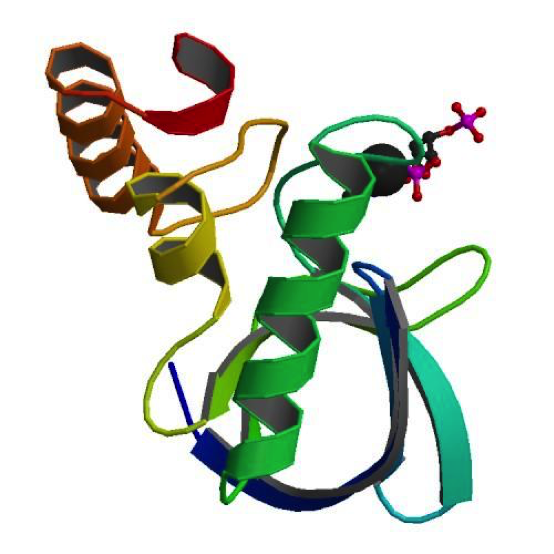
\includegraphics[width=\linewidth,keepaspectratio]{snase/ribbon-diagram}
 \caption[\lofimage{snase/ribbon-diagram}Ribbon diagram of Wild-Type SNase]{\label{fig:ribbon-diagram}This ribbon diagram shows the secondary structure of SNase. The $\alpha$-helix, positioned front and center from this perspective, acts a lid on the beta barrel (a beta sheet curved into a closed structure) beneath it. The interior of the beta barrel is hydrophobic, and the $\alpha$-helix helps keep water out. Change one residue in the middle of the helix creates a kink, effectively breaking the lid and ruining the stability of the folded structure.}
\end{figure}

In this chapter, we describe microrheology experiments on layers of wild-type and disordered SNase, adsorbed to the air--water interface. We speculate on the role of protein unfolding in the evolution of the mechanical response of the interface.

\section{Experimental Methods}

\subsection{Protein Fabrication}

The disordered SNase was fabricated by our collaborators in the lab of Prof. Bertrand Garcia-Moreno E. using the polymerase chain reaction (PCR). PCR is a standard, decades-old technique in biology, briefly review here for interested readers. To manufacture protein a certain engineered mutation, a fragment of DNA expressing the desired mutation is synthesized by chemically joining base pairs. A plasmid (circular ring of DNA) is obtained which largely compliments the fragment except at the site of the mutation. The primers and plasmids are combined in a soup of loose ribonucleotides and DNA polymerase, which marches along the chain and builds a DNA polymer along complemtary strands. The original primers are extended to full strands, and more full copies are made as the process proceeds. Finally, bacteria are made to imbibe the plasmids, and they manufacture mutated proteins in accordance with the mutated DNA. The product is purified and flash-frozen into droplet-sized beads for storage.

\subsection{Sample Preparation}

The frozen protein solution was thawed and diluted to 0.05 mg/ml in a 10 mM sodium phosphate buffer, pH 7.4. Then, following the protocol developed for the lysozyme study described in Chapter \ref{chap:lysozyme}, a volume of 0.5 ml was dispersed into a sample cell, where an air--water interface was formed. Colloidal probes were spread across the interface, dispersed in a solution of equal parts water and isopropyl alcohol.

\subsection{Active Microrheology}

Up to 15 separate rotations were performed at each age, using field strengths of 10--100 G, selected to match the stiffness of the layer so as to generate an observable wire rotation.


\section{Results}
\subsection{Wild-Type SNase Layer Evolution}

At early ages in the course of the layer's evolution, the wild-type layers were always found to exert a simple viscous drag on the wire. Their rotational trajectories were well described by Eq. (\ref{eq:sasha}),

\begin{equation*}
 \theta(t) = 2 \tan^{-1} \left[ \exp \left( -\frac{\mu B}{\zeta_r} (t-t_0) \right) \right].
\end{equation*}

where, as in Chapter \ref{chap:lysozyme}, $\mu$ is the wire's magnetic moment, $B$ is strength of the externally-applied magnetic field, $\zeta_r$ is a rotational drag coefficient, and $t_0$ is an experimental parameter that accounts for uncertainty in the time that the wire begins rotating in response to the field change. Figure \ref{fig:fitting-viscous-form}(a) shows rotational trajectories $\theta(t)$ in a wild-type layer at age $t_a=13$ minutes under field strengths of 10--35 G. Fitting Eq. (\ref{eq:sasha}) to each rotation gives a rate $K=\mu B/\zeta_r$, which is plotted against field strength $B$ in Figure \ref{fig:fitting-viscous-form}(b). The rotational drag coefficient $\zeta_r$ can be extracted from the slope of linear regression to $K(B)$. Then, using Eq. (\ref{eq:wire_zeta}), $\zeta_r = 1.48 L^2\eta_s$, we obtain the interfacial viscosity $\eta_s$. Thus, several wire rotations performed in succession at roughly the same age $t_a$ are reduced to a single number characterizing the linear shear rheology of the layer at that age. Figure \ref{fig:wt-viscosity-with-age} shows how, in several identically-prepared trials of wild-type SNase, the viscosity increased exponentially with the age of the layer over a wide range of ages. At ages later than those represented in this figure, the wire rotations changed qualitatively in a way that could no longer be explained in terms of simple viscous drag.

   \begin{figure}
    \centering
    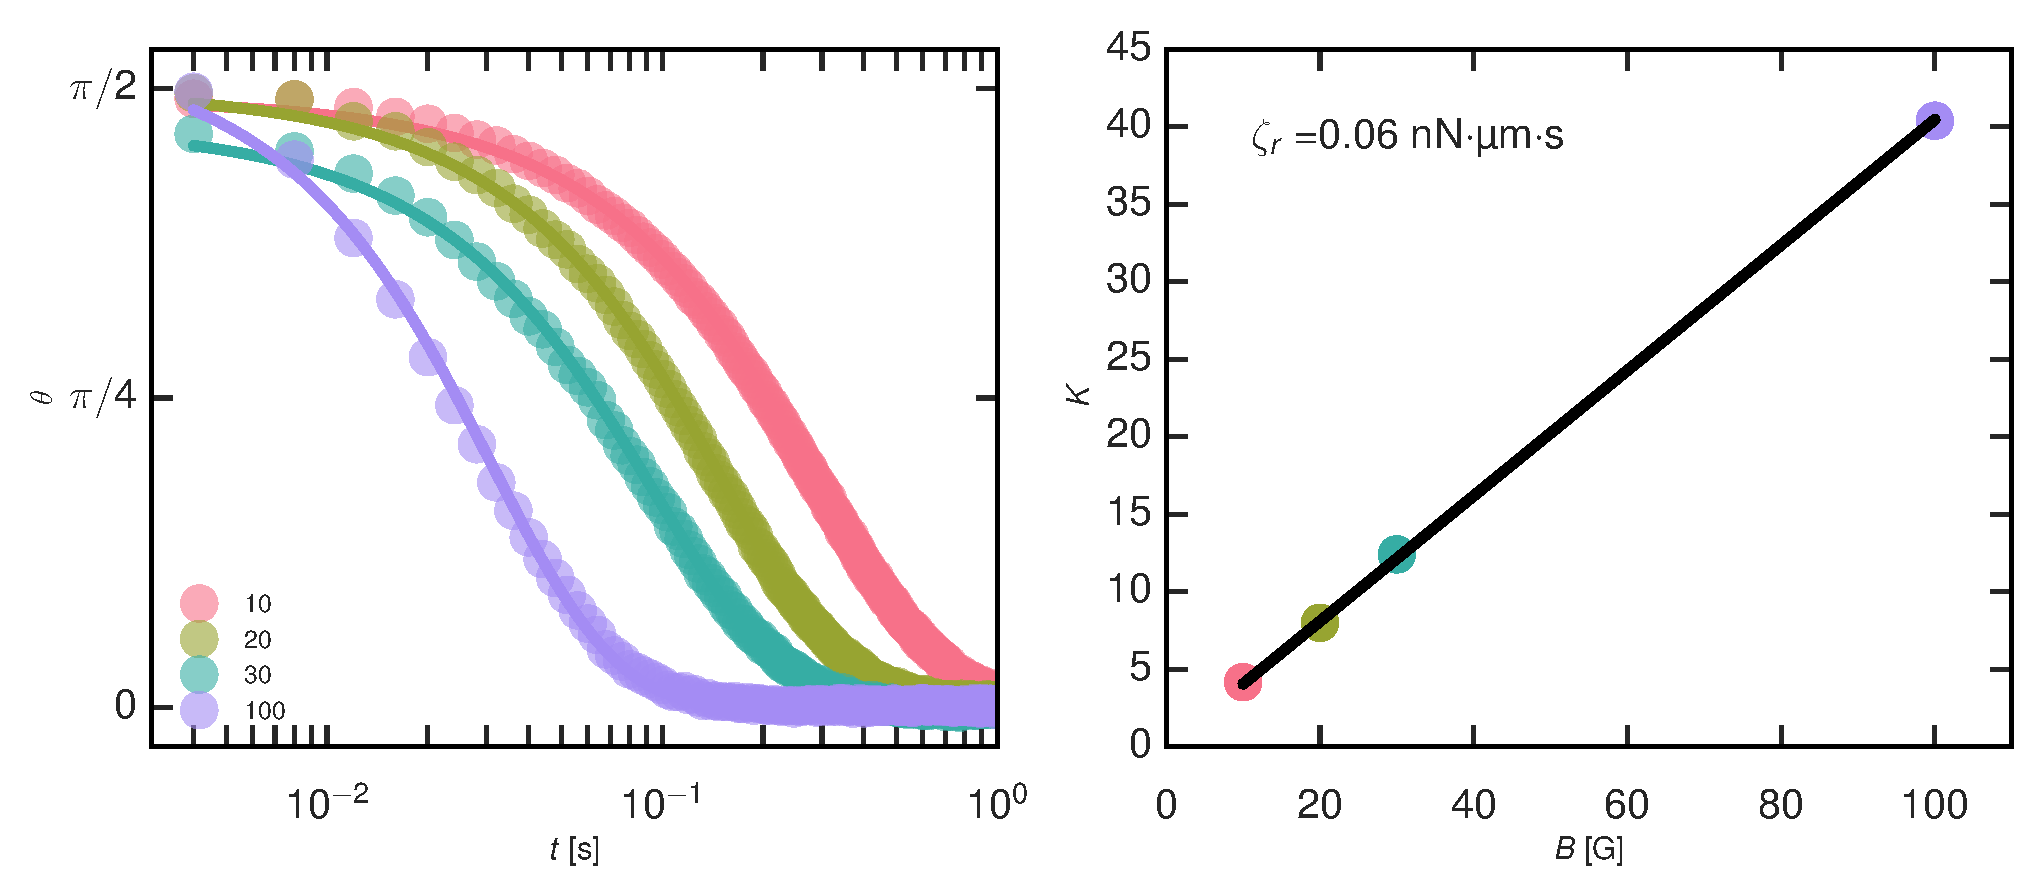
\includegraphics[width=\columnwidth]{snase/fitting-viscous-form} % from AT49 V5.ipynb
    \caption{\label{fig:fitting-viscous-form}(a) Rotational trajectories $\theta(t)$ of a wire in a wild-type SNase layer at age $t_a=13$ minutes under a 90$^\circ$ step change in magnetic field direction, under field strengths of 10--35 G. Eq. \ref{eq:sasha} is fit to each rotation, giving a rate $K=\mu B/\zeta_r$, which is plotted against field strength $B$ in (b). The slope of the linear regression to this data is used to compute $\zeta_r$.}
    \end{figure}

   \begin{figure}
    \centering
    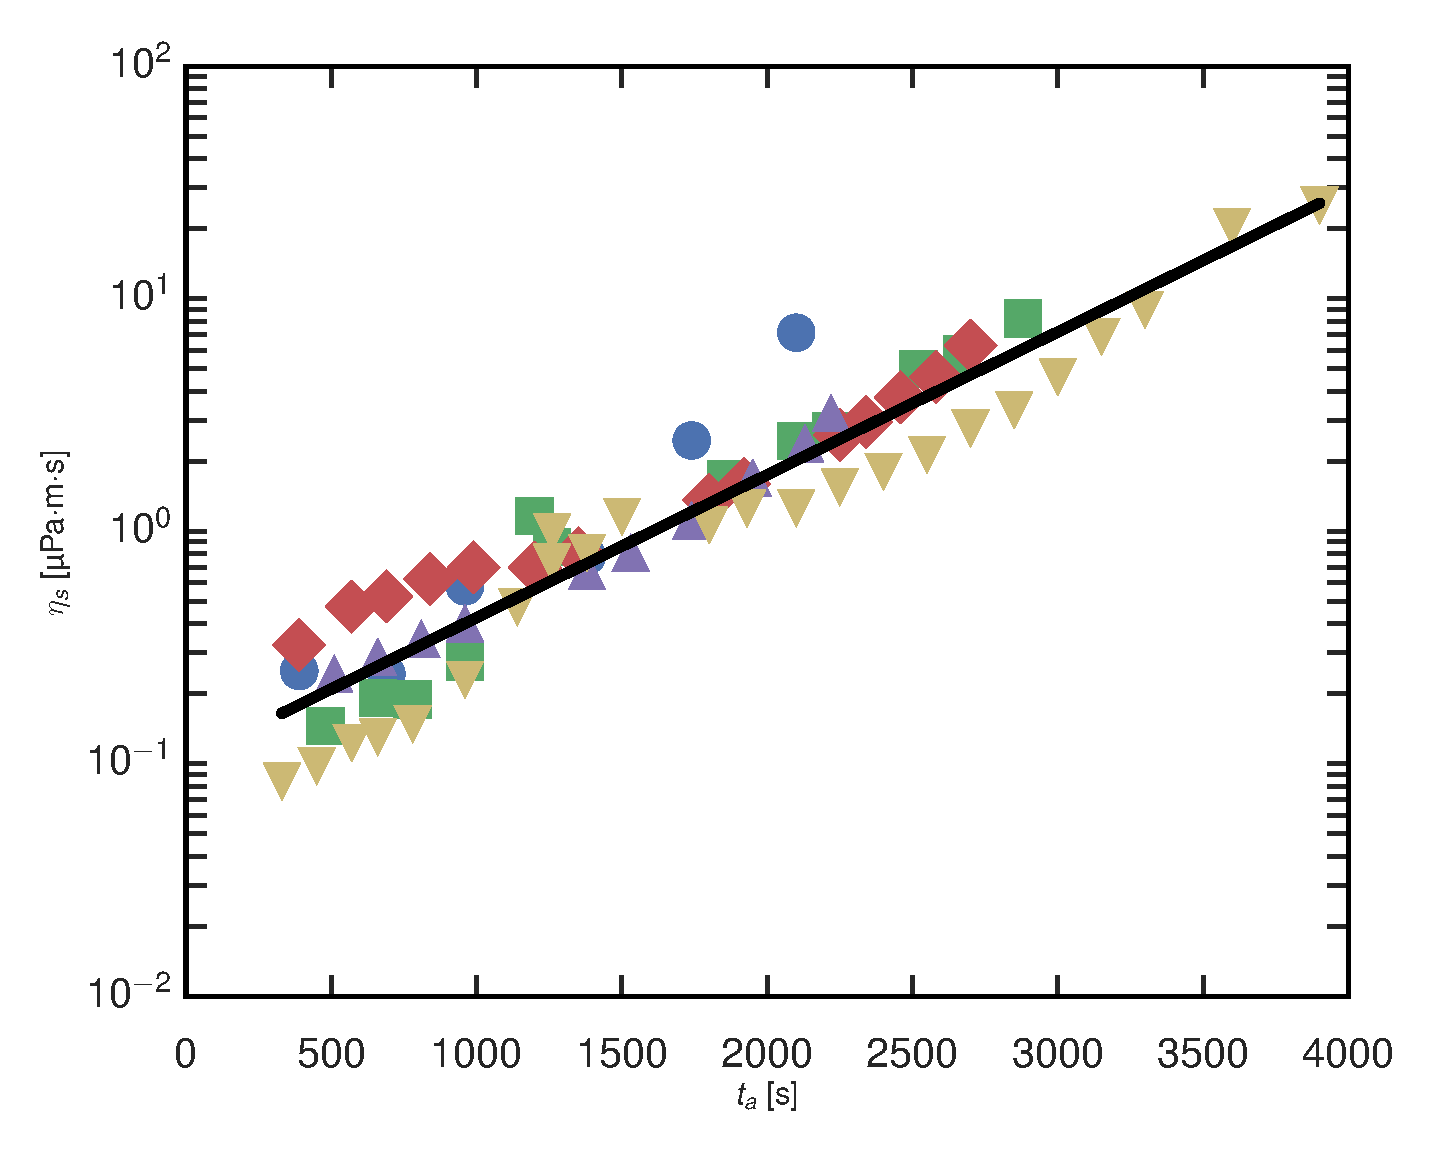
\includegraphics[width=\columnwidth]{snase/wt-viscosity-with-age}
    \caption{\label{fig:wt-viscosity-with-age}The interfacial viscosity of the layer, computed from wire rotation curves like those in Figure \ref{fig:fitting-viscous-form}, rose exponentially with layer age $t_a$. Data from several identically-prepared trails are shown, differentiated by plot markers.}
    \end{figure}
   

\subsection{Disordered SNase Layer Evolution}

The wire rotations in layers of disordered SNase showed more trail-to-trail variability. Some, like rotations in wild-type layers, were well-described by viscous drag at first. Others showed a more complex response from the beginning. Those that did show viscous behavior are characterized in Figure \ref{fig:dis-viscosity-with-age}. Notice that the change in viscosity is much less pronounced and occurs more slowly than in wild-type layers. (To aid the comparison, note that Figures \ref{fig:wt-viscosity-with-age} and \ref{fig:dis-viscosity-with-age} are plotted on the same scale.)

This apparent variability between trials may actually be a proxy for spatial variability in the layers. Straight, unaggregated wires are sufficiently sparse, and the evolution of the layer sufficiently fast, that it is not practical to observe more than one or two different wires in a given trial. Once a one or two usable wires are located in the layer, they must be carefully followed. There is no time to locate an ensemble of wires and regions to compare before the layer has aged dramatically. Thus, we speculate that the layers generated by disordered SNase exhibit mesoscale spatial heterogeneity that is not directly captured by our technique.

   \begin{figure}
    \centering
    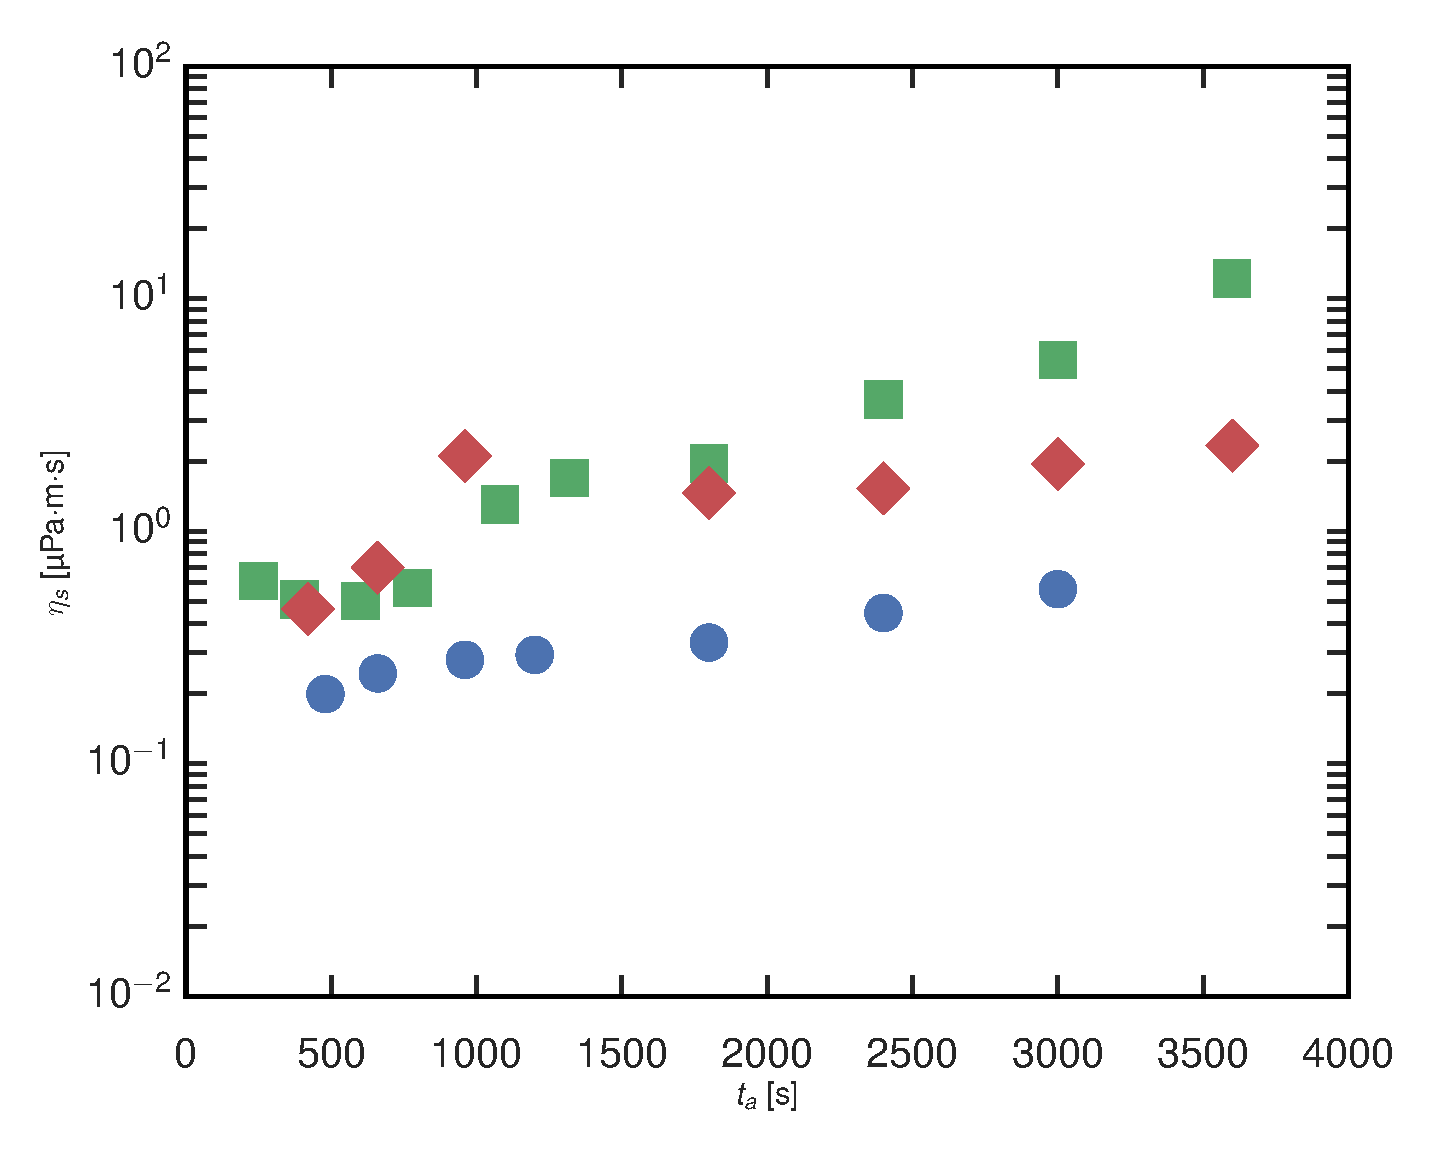
\includegraphics[width=\columnwidth]{snase/dis-viscosity-with-age}
    \caption{\label{fig:dis-viscosity-with-age}}
    \end{figure}


\section{Discussion \& Conclusion}

Although the analysis of these results is still in its early stages, we can already see that protein unfolding can play a dramatic role in the evolution of a layer's mechanical response during its formation.